% Method -- handbook section 2.3 requires this coverage
% Pipeline, baseline and main model, loss, and what was self-implemented.

\section{Method}

%----------------------------------------------------------
\begin{frame}{Pipeline}
\begin{figure}
    \centering
    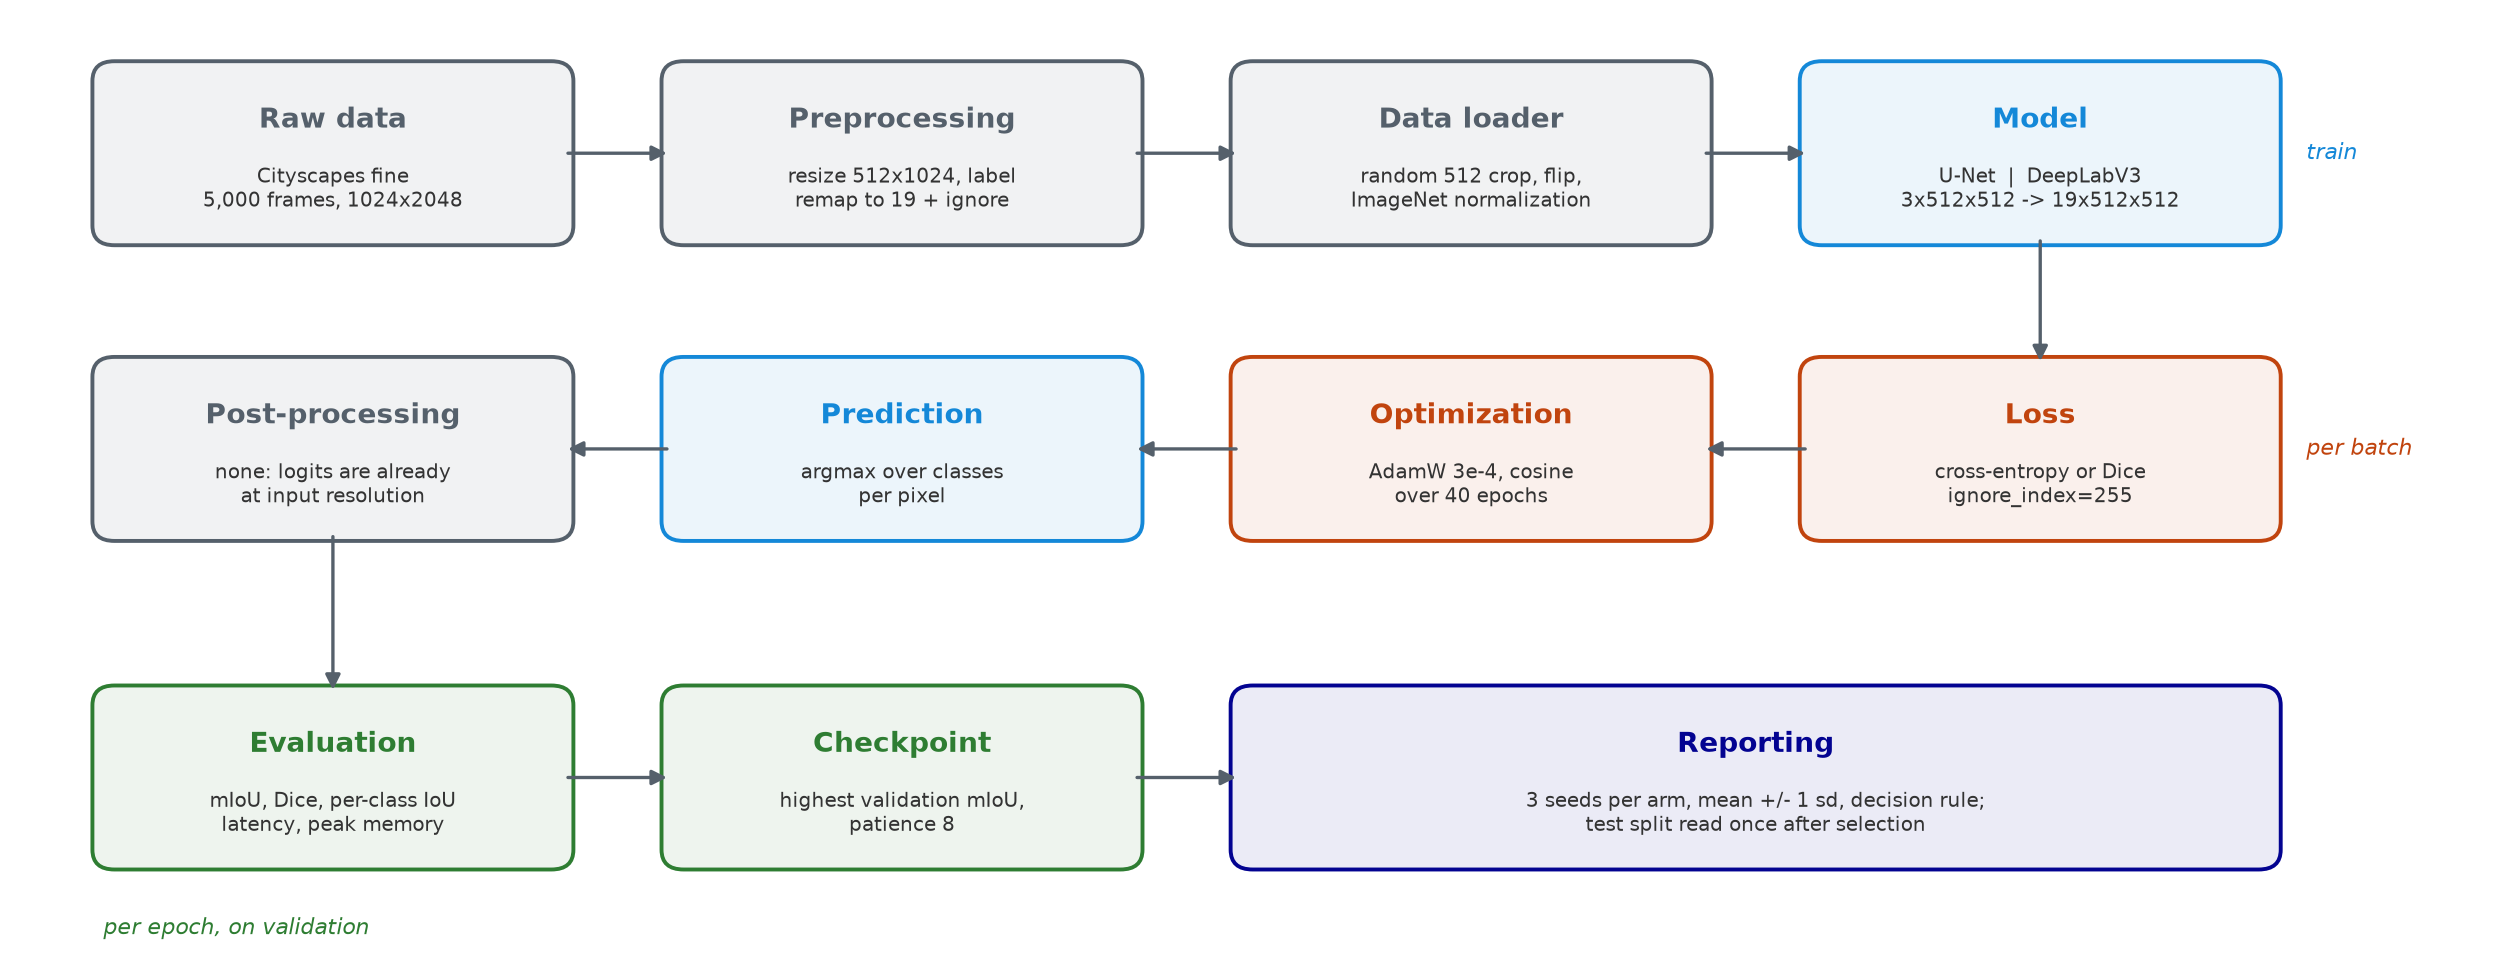
\includegraphics[width=0.90\textwidth]{../results/figures/pipeline.png}
\caption{The pipeline.}
\label{fig:pipeline}
\end{figure}

\vspace{-0.3cm}
\footnotesize
\begin{itemize}
    \item \textbf{Post-processing is empty by design:} both models emit logits at input
          resolution, so the prediction is an \texttt{argmax}; nothing is upsampled or smoothed.
    \item \textbf{Evaluation runs on two terms:} validation every epoch selects the checkpoint;
          test is read \emph{once}, after selection.
\end{itemize}
\end{frame}

%----------------------------------------------------------
\begin{frame}{U-Net, the Baseline}
\small
\begin{columns}[T]
\begin{column}{0.56\textwidth}
Written from scratch~\cite{ronneberger2015unet}; no pretrained weights. Base width 32, depth 4,
$7{,}763{,}635$ parameters.
\begin{equation*}
\begin{aligned}
    e_\ell &= \mathrm{DoubleConv}(\mathrm{MaxPool}_2(e_{\ell-1})) \\
    d_\ell &= \mathrm{DoubleConv}([\,\mathrm{ConvT}_2(d_{\ell+1});\, e_\ell\,])
\end{aligned}
\end{equation*}
\begin{itemize}
    \item Widths double, $32 \to 64 \to 128 \to 256$, bridged at 512.
    \item Convolutions carry \textbf{no bias}: each is followed by batch normalisation, which
          makes it redundant.
\end{itemize}
\end{column}
\begin{column}{0.42\textwidth}
\begin{block}{The skip connection is the architecture}
Four poolings take a 512-pixel crop to \textbf{32 pixels}, enough context to say \emph{what} a
region is, far too coarse to say \emph{where} its boundary runs.

Each decoder stage concatenates the encoder map of its own resolution, putting the upsampled
semantics back onto the detail that produced them.
\end{block}
\end{column}
\end{columns}
\end{frame}

%----------------------------------------------------------
\begin{frame}{DeepLabV3, the Pretrained Model}
\small
\begin{columns}[T]
\begin{column}{0.54\textwidth}
Torchvision DeepLabV3~\cite{chen2017deeplabv3} + MobileNetV3-Large~\cite{howard2019mobilenetv3},
pretrained on a COCO subset over an ImageNet backbone. $11{,}024{,}963$ parameters.
\begin{itemize}
    \item \textbf{No decoder:} dilated kernels keep the feature map at stride 8, and atrous
          spatial pyramid pooling gathers context at several rates in parallel.
    \item \textbf{Head replaced:} the published $1\times1$ convolution predicts 21 classes; ours
          predicts 19. Backbone and pooling module transfer unchanged.
\end{itemize}
\end{column}
\begin{column}{0.44\textwidth}
\begin{block}{Two details that matter}
\footnotesize
\textbf{Auxiliary head removed}, not computed and discarded, so training pays nothing for an output
no loss reads.

\textbf{Normalization taken from the weights}, not assumed. Feeding a differently normalised batch
to a pretrained backbone degrades it \emph{silently}, with no error to notice.
\end{block}
\end{column}
\end{columns}

\vspace{0.1cm}
\footnotesize
\textbf{Fine-tuning procedure:} one stage. The final convolution is replaced, then \emph{every}
parameter trains from epoch 1 at one learning rate, with no gradual unfreezing and no per-layer rates.
This is the same procedure the U-Net receives, so the comparison is between \emph{models}, not training schedules.
\end{frame}

%----------------------------------------------------------
\begin{frame}{Losses and Metrics}
\small
\begin{columns}[T]
\begin{column}{0.49\textwidth}
\textbf{Cross-entropy}, over labelled pixels only:
\begin{equation*}
    \mathcal{L} = -\frac{1}{|\Omega|}\!\!\sum_{(i,j) \in \Omega}\!\!
    \log \frac{\exp(z_{y_{ij}ij})}{\sum_c \exp(z_{cij})}
\end{equation*}
$\Omega = \{(i,j) : y_{ij} \neq 255\}$. Without it, the network would learn to reproduce the
bonnet of the recording vehicle.
\end{column}
\begin{column}{0.49\textwidth}
\textbf{Soft Dice}~\cite{milletari2016vnet}, the ablation arm:
\begin{equation*}
    \mathcal{L}_{\mathrm{Dice}} = 1 - \frac{1}{C}\sum_{c=1}^{C}
    \frac{2 \sum_\Omega p_{cij}\mathbf{1}[y_{ij}{=}c] + \varepsilon}
         {\sum_\Omega p_{cij} + \sum_\Omega \mathbf{1}[y_{ij}{=}c] + \varepsilon}
\end{equation*}
\end{column}
\end{columns}

\vspace{0.15cm}
\begin{itemize}
    \item \textbf{What they weight:} cross-entropy averages over \emph{pixels}, so a class counts
          in proportion to the ground it covers. Dice averages over \emph{classes}, so a pole
          counts as much as the road.
    \item \textbf{Metrics:} mIoU primary; Dice, per-class IoU, pixel accuracy secondary. All from
          one running $19 \times 19$ confusion matrix, because a validation pass holds 298M pixels, so
          masks are never concatenated.
    \item mIoU is a \texttt{nanmean}: a class absent from the ground truth is \emph{excluded},
          not scored zero.
\end{itemize}
\end{frame}

%----------------------------------------------------------
\begin{frame}{What Was Written, and What Was Imported}
\small
\begin{table}
\centering
\caption{Attribution.}
\begin{tabular}{ll}
\toprule
\textbf{Component} & \textbf{Origin} \\
\midrule
U-Net, Dice loss, confusion matrix and every metric & written by the group \\
Training loop, evaluation, experiment runner, figures & written by the group \\
DeepLabV3 and its pretrained weights & \texttt{torchvision.models.segmentation} \\
Layer primitives, cross-entropy, AdamW, cosine schedule & PyTorch~\cite{paszke2019pytorch} \\
labelId $\rightarrow$ trainId table & \texttt{cityscapesscripts} \\
Plots & matplotlib \\
\bottomrule
\end{tabular}
\end{table}
\end{frame}
